\section{Tests realisés pour valider le fonctionnement du TP}
\bframe{
Les tests réalisés ont étés les suivants:

%\item \code{./digest -f file1 file2 ...[-t <hashMethod>]} \\
{\scriptsize \code{./ultra-cp dossier\_1 [[$\cdots$ dossier\_n] [fichier\_1 $\cdots$
    fichier\_n]]}\\

    $\qquad \qquad \qquad \qquad \qquad$ \code{[destination] [-a] [-f] }}

Selon les utilisations suivantes: (commentaire copié du code)
\begin{enumerate}
    \item[1.] Just 1 file/folder $\Rightarrow$ print/ls contents
    \item[2.] If only 2 files are given $\Rightarrow$ create/replace the file
    \item[3.] If multiple files \& folder and \quo{dest} exists $\Rightarrow$ create/replace architecture in \quo{dest}
    \item[4.] If -a is passed, change the permissions
    \item[5.] If -f is passed, links are copied as links (stored in optional state)
\end{enumerate}

}

\bframe{
    \vspace{-0.2cm}
    {\scriptsize Soit le dossier \code{res/} contenant les fichiers suivants:}
    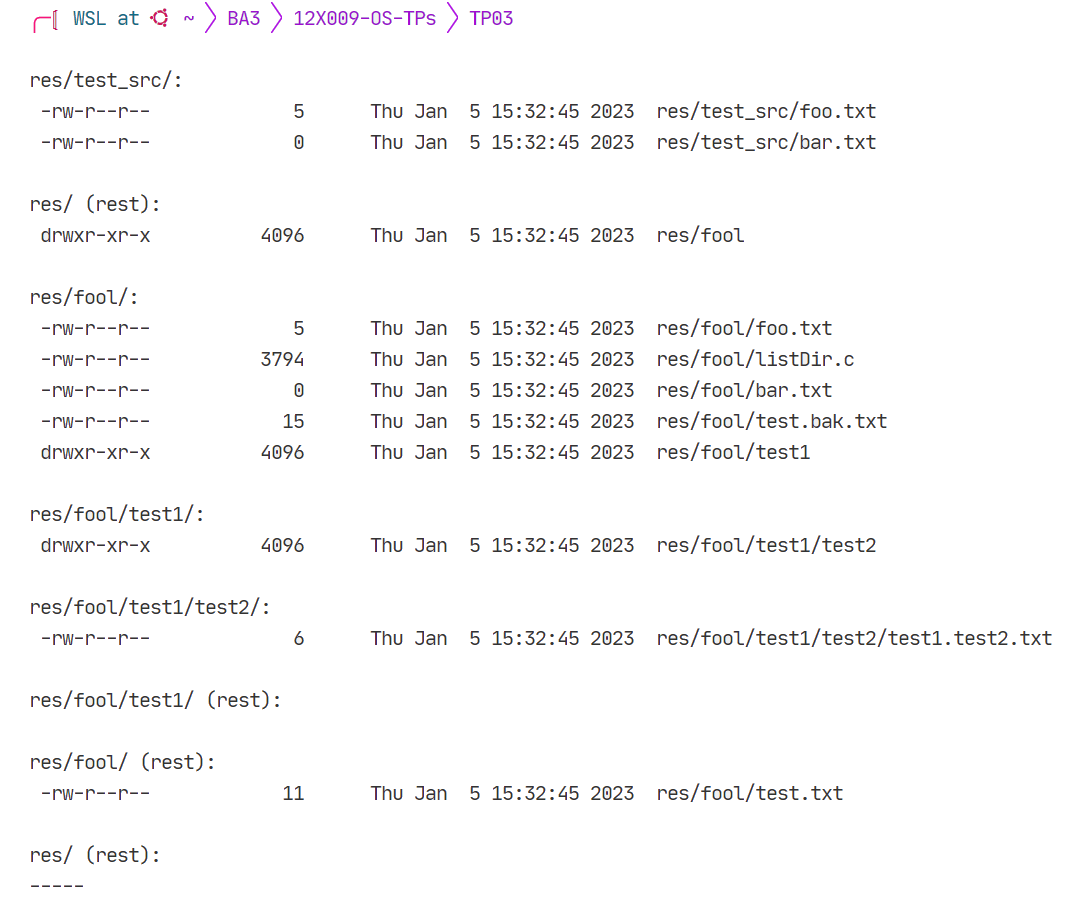
\includegraphics[scale=0.48]{images/os-tp3-prez-resDir2.png}
}

\bframe{
    Les tests suivants ont été réalisés:
  
  \begin{enumerate}
      \item \code{./ultra-cp res/fool tmp}
      \item \code{./ultra-cp res/fool/bar.txt tmp}
      \item \code{./ultra-cp  res/test\_src/foo.txt}
      \item \code{./ultra-cp  res/test\_src/foo.txt foo}
      \item \code{./ultra-cp res/test\_src/bar.txt res/test\_src/foo.txt  res/test\_src res/fool}
   
  \end{enumerate}
}


\bframe{
    Les tests suivants ont été réalisés:
  
  \begin{enumerate}
      \item \code{./ultra-cp res/fool tmp -f}
      \item \code{./ultra-cp res/fool/bar.txt tmp.txt}
      \item \code{./ultra-cp  res/test\_src/foo.txt}
      \item \code{./ultra-cp  res/test\_src/foo.txt foo}
      \item \code{./ultra-cp res/test\_src/bar.txt res/test\_src/foo.txt} \\
      $\qquad \qquad \quad$ \code{res/test\_src res/fool -f}
  \end{enumerate}
  La dernière commande donnant l'output suivant:
}

\bframe{
    \vspace{-0.2cm}
    \includegraphics[scale=0.48]{images/os-tp3-prez-lastTest.png}
}


